\chapter{Introduction}\label{chap:intro}
% {First paragraph: problem definition + applications
\begin{figure*}[b!]
	\centering
	\setlength\tabcolsep{3pt}
	\begin{tabular}{ccc}
		%	\rotatebox{90}{    \, FAUST} &
		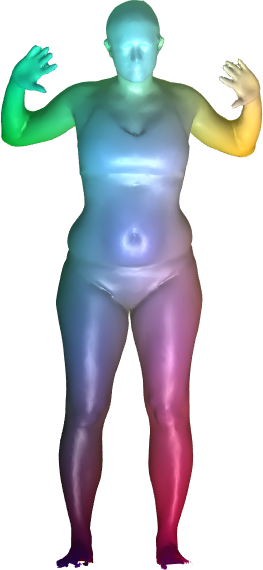
\includegraphics[width=0.1\textwidth]{figures/test_scan_031_test_scan_034_PFM.png}  &
		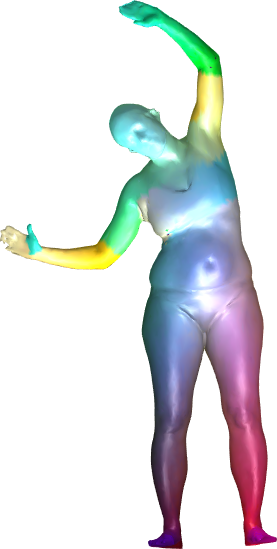
\includegraphics[width=0.1333\textwidth]{figures/test_scan_034.png} &
		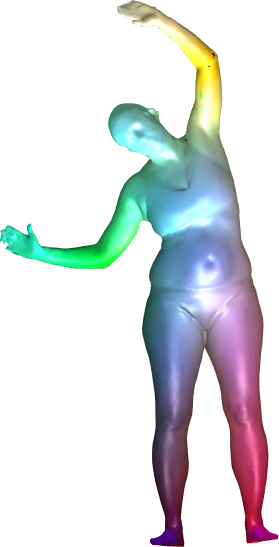
\includegraphics[width=0.1333\textwidth]{figures/test_scan_031_test_scan_034.png}\\
		\multicolumn{3}{c}{(a) large deformations}\\
		%	 \rotatebox{90}{    \, SHREC'16A} &
		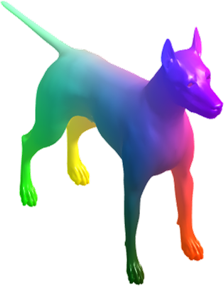
\includegraphics[scale=0.5]{figures/dog_base.png}&
		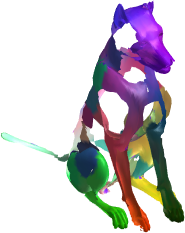
\includegraphics[scale=0.55]{figures/holes_dog_shape_25_PFM.png}&
		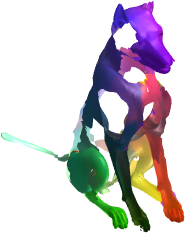
\includegraphics[scale=0.55]{figures/holes_dog_shape_25.png}\\
		\multicolumn{3}{c}{(b) partiality}\\
		%	\rotatebox{90}{    \, SHREC'16B} &
		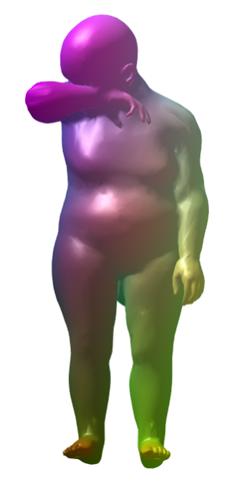
\includegraphics[width=0.12\textwidth]{figures/Top1Base.png} &
		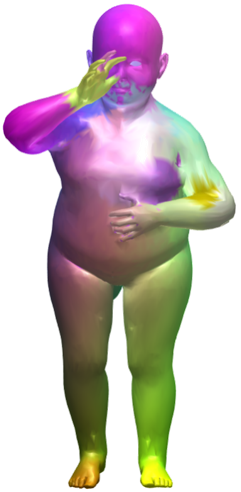
\includegraphics[width=0.12\textwidth]{figures/Top1PFM.png} &
		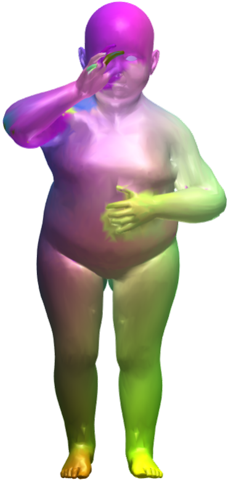
\includegraphics[width=0.12\textwidth]{figures/Top1DDIS.png} \\
		\multicolumn{3}{c}{(b) topological noise}\\\\
		Input & Rodola'17\cite{rodola2017partial} & Ours \\
	\end{tabular}
	\caption{{\textbf{Challenging correspondences.}}  
		Corresponding vertices are colored similarly.
		(a) While the corresponding arms are switched in~\cite{rodola2017partial}, our algorithm manages to match the arms correctly.
		(b) When given a highly partial model of a dog as input, our algorithm manages to match its four dog's legs correctly.
		(c) The right hand is well matched by our algorithm. 
	}
	\label{fig:teaser}
\end{figure*}

Shape correspondence is a fundamental problem in computer vision and computer graphics, both in 2D and in 3D.
Numerous applications require robust correspondences, for instance in animation, reconstruction, and shape analysis~\cite{van2011survey}.
The focus of this paper is on shape correspondence between meshes in 3D.




Finding correspondences between shapes is highly challenging, even when the objects are rigid and full~\cite{Biasotti03,barequet1997partial,mellado2014super,Zeng_2017_CVPR}. 
This paper, however, addresses the problem of shape correspondence, when the following additional challenges are added (see Figure~\ref{fig:teaser}):
(1)~The objects may have gone through non-rigid deformations~\cite{dubrovina2010matching,lipman2009mobius,Maron:2016:PRV:2897824.2925913,solomon2016entropic,vestner2017product}; 
(2)~only part of the shape is given and should be  matched to the correct region within the full shape ({\em partiality})~\cite{biasotti2006sub,itskovich2011surface,rodola2017partial,sahilliouglu2012minimum},  and
(3)~non-adjacent parts of the surfaces intersect~\cite{chen2015robust,litany2017fully,vanKaick:2013:BMP:2771539.2771553,vestner2017efficient} ({\em topological noise}).
All of the above frequently occur in real world scenarios.

% second paragraph: related work in short
Previous approaches have focused on minimization of some distortion criteria, of either point-wise shape descriptors~\cite{litany2017fully,rodola2017partial}, pair-wise shape descriptors~\cite{sahilliouglu2012minimum}, or the combination of both~\cite{vestner2017efficient}.
Impressive result have been exhibited , yet some downfalls still exist.
This is in particular evident in the three cases mentioned above, in particular when the  deformation is extreme, when partiality is severe, and in many cases of topological noise.

Some recent approaches have utilized deep neural networks~\cite{boscaini2016learning,litany2017deep,Masci:2015:GCN:2919341.2920992,monti2017geometric}.
These show a lot of promise on a couple of full-shape benchmarks. 
In~\cite{boscaini2016learning} the results are analyzed also for a  partial correspondence benchmark; 
we will show that our method outperforms their results.
All these methods require a significant amount of labeled training data, which is currently difficult to acquire. 

The algorithm proposed in this paper belongs to the first class of algorithms, which does not utilize deep learning.
It proposes a novel similarity function, which analyzes the nearest neighbor field in vertex shape descriptor space.
That is to say, for each vertex of a source mesh we find the nearest neighbor in the target mesh, in terms of a specific shape descriptor and a distance function.
Rather than minimizing some function of distances, we analyze statistics of this field.
The statistical nature of our method lets it ignore outliers, which are the source of unreliability in some other methods.
Specifically, the statistics we are concerned about regard two aspects of the nearest neighbor field:
(1) the diversity of the field, i.e. how many different matches the nearest neighbor field contains, and
(2) preservation of pairwise distances of the matches in the nearest neighbor field.

We have tested our method on the two challenging benchmarks of {\em SHREC'16}, the one that contains partial deformed shapes~\cite{cosmo2016shrec} and and the one that contains deformed shapes with topological noise~\cite{lahner2016shrec}.
We exhibit the benefit of our method both qualitatively (Figure~\ref{fig:teaser}) and quantitatively.
In particular, our method obtains a $10$-$20\%$ improvement over the state-of-the-art on the first dataset and is competitive on the second.
In addition, we also show qualitative results on the FAUST dataset~\cite{bogo2014faust}.

Hence, our contribution is twofold.
\begin{enumerate}
	\item
	We introduce a new approach for finding correspondences between given meshes, which is robust to deformations, partiality and topological noise.
	The novelty of our approach is relying on properties of the nearest-neighbor field.
	\item
	We demonstrate the benefits of our algorithm on the commonly-used benchmarks, both quantitatively and qualitatively.
\end{enumerate}
